\chapter{Conclusie}
\label{chap:conclusion}

Aan de hand van de analyses uit de vorige hoofdstukken is te zien dat de BFS methode het beste werkt bij de geanalyseerde grafen. 

\begin{table}[h]
 \begin{tabularx}{\linewidth}{| l | X | X | X |}
  \hline
   Graaf 1 & DFS & BFS & DIJKSTRA \\
   \hline
  Bezochte knopen & 17 & 11 & 18 \\
 \hline
  Bezochte kanten & 18 & 15 & 36 \\
\hline
 Iteraties & 5 & 4 & 4 \\
 \hline
 Tijd & 70.261 ns & 57.061 ns & 151.140 ns. \\
 \hline
 \end{tabularx}
 \label{tbl:concl_graaf1}
 \caption{Resultaten voor graaf 1}
\end{table}

\begin{table}[h]
 \begin{tabularx}{\linewidth}{| l | X | X | X |}
  \hline
   Graaf 2 & DFS & BFS & DIJKSTRA \\
   \hline
  Bezochte knopen & 31 & 29 & 43 \\
 \hline
  Bezochte kanten & 42 & 48 & 123 \\
\hline
 Iteraties & 7 & 7 & 6 \\
 \hline
 Tijd & 124.450 ns. & 149.954 ns. & 361.438 ns. \\
 \hline
 \end{tabularx}
 \label{tbl:concl_graaf2}
 \caption{Resultaten voor graaf 2}
\end{table}

\clearpage

\begin{figure}[h]
 \centering
 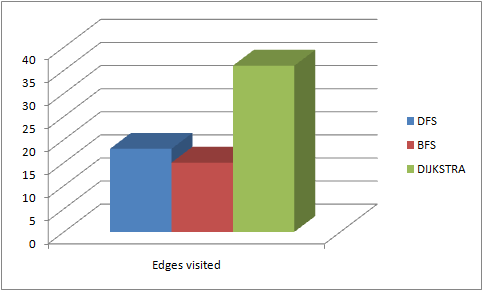
\includegraphics[width=0.5\linewidth]{conclusion/graph1_edges}
 \caption{Bezochte kanten van graaf 1}
 \label{fig:graph1_edges}
\end{figure}

\begin{figure}[h]
 \centering
 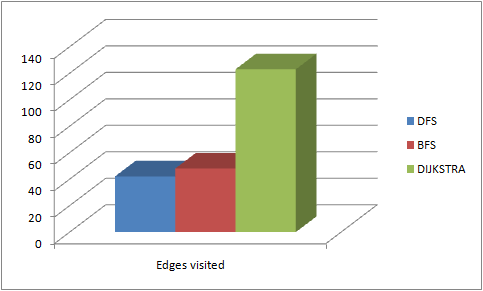
\includegraphics[width=0.5\linewidth]{conclusion/graph2_edges}
 \caption{Bezochte kanten van graaf 2}
 \label{fig:graph2_edges}
\end{figure}

\begin{figure}[h]
 \centering
 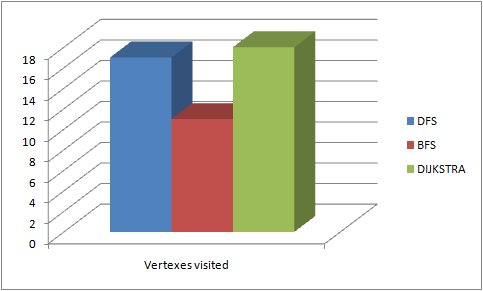
\includegraphics[width=0.5\linewidth]{conclusion/graph1_vertexes}
 \caption{Bezochte knopen van graaf 1}
 \label{fig:graph1_vertexes}
\end{figure}

\begin{figure}[h]
 \centering
 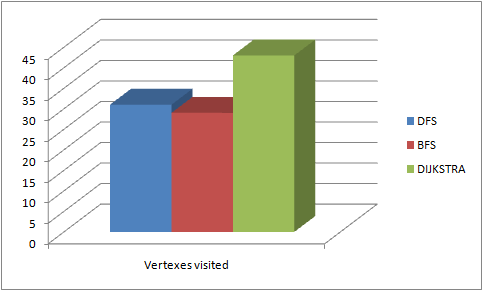
\includegraphics[width=0.5\linewidth]{conclusion/graph2_vertex}
 \caption{Bezochte knopen van graaf 2}
 \label{fig:graph2_vertexes}
\end{figure}

\begin{figure}[h]
 \centering
 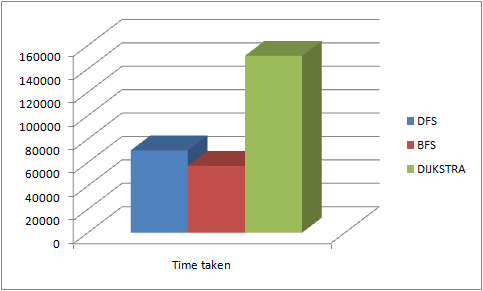
\includegraphics[width=0.5\linewidth]{conclusion/graph1_time}
 \caption{Tijd voor graaf 1}
 \label{fig:graph1_time}
\end{figure}

\begin{figure}[h]
 \centering
 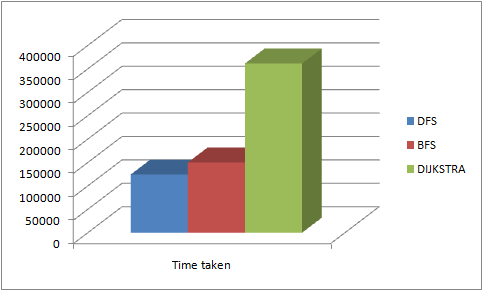
\includegraphics[width=0.5\linewidth]{conclusion/graph2_time}
 \caption{Tijd voor graaf 2}
 \label{fig:graph2_time}
\end{figure}